\documentclass{article}
\usepackage[utf8]{inputenc}
\usepackage[top=1in]{geometry}
\usepackage{graphicx}
\usepackage{booktabs}
\usepackage{amsmath}
% Calligraphic fonts
\newcommand{\calA}{{\cal A}}
\newcommand{\calB}{{\cal B}}
\newcommand{\calC}{{\cal C}}
\newcommand{\calD}{{\cal D}}
\newcommand{\calE}{{\cal E}}
\newcommand{\calF}{{\cal F}}
\newcommand{\calG}{{\cal G}}
\newcommand{\calH}{{\cal H}}
\newcommand{\calI}{{\cal I}}
\newcommand{\calJ}{{\cal J}}
\newcommand{\calK}{{\cal K}}
\newcommand{\calL}{{\cal L}}
\newcommand{\calM}{{\cal M}}
\newcommand{\calN}{{\cal N}}
\newcommand{\calO}{{\cal O}}
\newcommand{\calP}{{\cal P}}
\newcommand{\calQ}{{\cal Q}}
\newcommand{\calR}{{\cal R}}
\newcommand{\calS}{{\cal S}}
\newcommand{\calT}{{\cal T}}
\newcommand{\calU}{{\cal U}}
\newcommand{\calV}{{\cal V}}
\newcommand{\calW}{{\cal W}}
\newcommand{\calX}{{\cal X}}
\newcommand{\calY}{{\cal Y}}
\newcommand{\calZ}{{\cal Z}}

% Sets:
\newcommand{\setA}{\textsf{A}}
\newcommand{\setB}{\textsf{B}}
\newcommand{\setC}{\textsf{C}}
\newcommand{\setD}{\textsf{D}}
\newcommand{\setE}{\textsf{E}}
\newcommand{\setF}{\textsf{F}}
\newcommand{\setG}{\textsf{G}}
\newcommand{\setH}{\textsf{H}}
\newcommand{\setI}{\textsf{I}}
\newcommand{\setJ}{\textsf{J}}
\newcommand{\setK}{\textsf{K}}
\newcommand{\setL}{\textsf{L}}
\newcommand{\setM}{\textsf{M}}
\newcommand{\setN}{\textsf{N}}
\newcommand{\setO}{\textsf{O}}
\newcommand{\setP}{\textsf{P}}
\newcommand{\setQ}{\textsf{Q}}
\newcommand{\setR}{\textsf{R}}
\newcommand{\setS}{\textsf{S}}
\newcommand{\setT}{\textsf{T}}
\newcommand{\setU}{\textsf{U}}
\newcommand{\setV}{\textsf{V}}
\newcommand{\setW}{\textsf{W}}
\newcommand{\setX}{\textsf{X}}
\newcommand{\setY}{\textsf{Y}}
\newcommand{\setZ}{\textsf{Z}}

% Vectors
\newcommand{\bfa}{\mathbf{a}}
\newcommand{\bfb}{\mathbf{b}}
\newcommand{\bfc}{\mathbf{c}}
\newcommand{\bfd}{\mathbf{d}}
\newcommand{\bfe}{\mathbf{e}}
\newcommand{\bff}{\mathbf{f}}
\newcommand{\bfg}{\mathbf{g}}
\newcommand{\bfh}{\mathbf{h}}
\newcommand{\bfi}{\mathbf{i}}
\newcommand{\bfj}{\mathbf{j}}
\newcommand{\bfk}{\mathbf{k}}
\newcommand{\bfl}{\mathbf{l}}
\newcommand{\bfm}{\mathbf{m}}
\newcommand{\bfn}{\mathbf{n}}
\newcommand{\bfo}{\mathbf{o}}
\newcommand{\bfp}{\mathbf{p}}
\newcommand{\bfq}{\mathbf{q}}
\newcommand{\bfr}{\mathbf{r}}
\newcommand{\bfs}{\mathbf{s}}
\newcommand{\bft}{\mathbf{t}}
\newcommand{\bfu}{\mathbf{u}}
\newcommand{\bfv}{\mathbf{v}}
\newcommand{\bfw}{\mathbf{w}}
\newcommand{\bfx}{\mathbf{x}}
\newcommand{\bfy}{\mathbf{y}}
\newcommand{\bfz}{\mathbf{z}}


\newcommand{\bfalpha}{\boldsymbol{\alpha}}
\newcommand{\bfbeta}{\boldsymbol{\beta}}
\newcommand{\bfgamma}{\boldsymbol{\gamma}}
\newcommand{\bfdelta}{\boldsymbol{\delta}}
\newcommand{\bfepsilon}{\boldsymbol{\epsilon}}
\newcommand{\bfzeta}{\boldsymbol{\zeta}}
\newcommand{\bfeta}{\boldsymbol{\eta}}
\newcommand{\bftheta}{\boldsymbol{\theta}}
\newcommand{\bfiota}{\boldsymbol{\iota}}
\newcommand{\bfkappa}{\boldsymbol{\kappa}}
\newcommand{\bflambda}{\boldsymbol{\lambda}}
\newcommand{\bfmu}{\boldsymbol{\mu}}
\newcommand{\bfnu}{\boldsymbol{\nu}}
\newcommand{\bfomicron}{\boldsymbol{\omicron}}
\newcommand{\bfpi}{\boldsymbol{\pi}}
\newcommand{\bfrho}{\boldsymbol{\rho}}
\newcommand{\bfsigma}{\boldsymbol{\sigma}}
\newcommand{\bftau}{\boldsymbol{\tau}}
\newcommand{\bfupsilon}{\boldsymbol{\upsilon}}
\newcommand{\bfphi}{\boldsymbol{\phi}}
\newcommand{\bfchi}{\boldsymbol{\chi}}
\newcommand{\bfpsi}{\boldsymbol{\psi}}
\newcommand{\bfomega}{\boldsymbol{\omega}}
\newcommand{\bfxi}{\boldsymbol{\xi}}
\newcommand{\bfell}{\boldsymbol{\ell}}

% Matrices
\newcommand{\bfA}{\mathbf{A}}
\newcommand{\bfB}{\mathbf{B}}
\newcommand{\bfC}{\mathbf{C}}
\newcommand{\bfD}{\mathbf{D}}
\newcommand{\bfE}{\mathbf{E}}
\newcommand{\bfF}{\mathbf{F}}
\newcommand{\bfG}{\mathbf{G}}
\newcommand{\bfH}{\mathbf{H}}
\newcommand{\bfI}{\mathbf{I}}
\newcommand{\bfJ}{\mathbf{J}}
\newcommand{\bfK}{\mathbf{K}}
\newcommand{\bfL}{\mathbf{L}}
\newcommand{\bfM}{\mathbf{M}}
\newcommand{\bfN}{\mathbf{N}}
\newcommand{\bfO}{\mathbf{O}}
\newcommand{\bfP}{\mathbf{P}}
\newcommand{\bfQ}{\mathbf{Q}}
\newcommand{\bfR}{\mathbf{R}}
\newcommand{\bfS}{\mathbf{S}}
\newcommand{\bfT}{\mathbf{T}}
\newcommand{\bfU}{\mathbf{U}}
\newcommand{\bfV}{\mathbf{V}}
\newcommand{\bfW}{\mathbf{W}}
\newcommand{\bfX}{\mathbf{X}}
\newcommand{\bfY}{\mathbf{Y}}
\newcommand{\bfZ}{\mathbf{Z}}


\newcommand{\bfGamma}{\boldsymbol{\Gamma}}
\newcommand{\bfDelta}{\boldsymbol{\Delta}}
\newcommand{\bfTheta}{\boldsymbol{\Theta}}
\newcommand{\bfLambda}{\boldsymbol{\Lambda}}
\newcommand{\bfPi}{\boldsymbol{\Pi}}
\newcommand{\bfSigma}{\boldsymbol{\Sigma}}
\newcommand{\bfUpsilon}{\boldsymbol{\Upsilon}}
\newcommand{\bfPhi}{\boldsymbol{\Phi}}
\newcommand{\bfPsi}{\boldsymbol{\Psi}}
\newcommand{\bfOmega}{\boldsymbol{\Omega}}


% Blackboard Bold:
\newcommand{\bbA}{\mathbb{A}}
\newcommand{\bbB}{\mathbb{B}}
\newcommand{\bbC}{\mathbb{C}}
\newcommand{\bbD}{\mathbb{D}}
\newcommand{\bbE}{\mathbb{E}}
\newcommand{\bbF}{\mathbb{F}}
\newcommand{\bbG}{\mathbb{G}}
\newcommand{\bbH}{\mathbb{H}}
\newcommand{\bbI}{\mathbb{I}}
\newcommand{\bbJ}{\mathbb{J}}
\newcommand{\bbK}{\mathbb{K}}
\newcommand{\bbL}{\mathbb{L}}
\newcommand{\bbM}{\mathbb{M}}
\newcommand{\bbN}{\mathbb{N}}
\newcommand{\bbO}{\mathbb{O}}
\newcommand{\bbP}{\mathbb{P}}
\newcommand{\bbQ}{\mathbb{Q}}
\newcommand{\bbR}{\mathbb{R}}
\newcommand{\bbS}{\mathbb{S}}
\newcommand{\bbT}{\mathbb{T}}
\newcommand{\bbU}{\mathbb{U}}
\newcommand{\bbV}{\mathbb{V}}
\newcommand{\bbW}{\mathbb{W}}
\newcommand{\bbX}{\mathbb{X}}
\newcommand{\bbY}{\mathbb{Y}}
\newcommand{\bbZ}{\mathbb{Z}}




\title{Number system and conversions (section 1.4 of textbook)}
\author{Vikas Dhiman}
\newtheorem{prob}{Problem}

\newcommand{\bx}{\bar{x}}
\newcommand{\by}{\bar{y}}
\newcommand{\bz}{\bar{z}}
\newcommand{\bA}{\bar{A}}
\newcommand{\bB}{\bar{B}}
\newcommand{\bC}{\bar{C}}
\begin{document}
\maketitle

\section{Place value number system}

A decimal number 1342 can be written as
\begin{align*}
  1342&=1\times1000 + 3\times100 + 4\times10 + 2\times1
        \\
      &=1\times10^3 + 3\times10^2+4\times10^1 + 2\times10^0.
\end{align*}

Decimal numbers are said to be of base (or radix) 10. One can generalize this
idea to arbitrary base (or radix) $r$. The same number expressed in some other
base $r$ will have a very different value:
\begin{align*}
  (1342)_r &=1\times r^3 + 3\times r^2+4\times r^1 + 2\times r^0.
\end{align*}

In general the \emph{value} of a arbitrary $n$-digit number $d_{n-1}d_{n-2}
\dots d_1 d_0$ in base $r$ is:
\begin{align*}
  (d_{n-1}d_{n-2} \dots d_1 d_0)_r &=d_{n-1} \times r^{n-1} + d_{n-2}\times r^{n-2}+ \dots + d_1\times r^1 + d_0\times r^0 &= \sum_{k=0}^{n-1} d_k r^k
\end{align*}
Each digit value is always smaller than base $d_k <= r-1$.

\section{Binary numbers}

Numbers with base $2$ are called binary numbers. For example, the number
$(10110)_2$ has value:
\begin{align*}
  (10110)_2 &= 1 \times 2^4+ 0 \times 2^3 + 1\times 2^2 + 1 \times 2^1+ 0\times 2^0
              \\
            &= 22.
\end{align*}

\begin{prob}
  Convert the following binary numbers to decimal: $(11110)_2$, $(100111)_2$.
\end{prob}
\vspace{10em}

\paragraph{Conversion from decimal to binary}
The value is in decimal because we find it easy to do calculations in decimal
numbers. Decimal values can be converted back to Binary representation by
\emph{repeated division} by 2 while noting down the remainder. Allow me
to use $/$ sign to denote both quotient and remainder after division. Let's convert $(22)_{10}$
back to binary: 

\begin{align*}
  22 / 2 &= (11, 0) & \text{ 11 is the quotient and 0 is the remainder} \\
  11 / 2 &= (5, 1) & \text{5 is the quotient and 1 is the remainder}\\
  5 / 2 &= (2, 1) & \\ 
  2 / 2 &= (1, 0) & \\
  1 / 2 &= (0, 1) &
\end{align*}

Read the remainders from bottom to top and right them as left to right, to form the resultant binary number $(22)_{10} = (10110)_2$.

\begin{prob}
Find the binary representation for decimal numbers: $123$ and $89$. Show your work.
\end{prob}
\vspace{10em}


\section{Hexadecimal numbers}
Numbers with base $16$ are called Hexadecimal numbers. From 0 to 9 the symbols
are same as decimal numbers. From 10 to 15, Hexadecimal numbers use A to F.
\[ A = 10, B = 11, C = 12, D = 13, E = 14, F = 15 \]. Example, $(10AD)_{16} = 1
\times 16^3 + 10 \times 16^1 + 13 = 4096 + 160 + 13 = 4269$.

\section{Octal numbers}
Numbers with base $8$ are called octal numbers. Example, $(354)_8 = 3 \times 8^2
+ 5 \times 8 + 4 = 192 + 40 + 4 = 236$.



\section{Hexadecimal/octal to binary and vice-versa}
Normally, if you have to convert between a number of base $r_1$ to a number of
base $r_2$, we will have to convert it via decimal numbers. Convert from base
$r_1$ to decimal and then from decimal to $r_2$.

Since Hexadecimal base $16$ is an exact power of $2$ ($16 = 2^4$). Conversion
between Hexadecimal to binary is easy. You can group 4 binary digits from right
to left and convert each group of 4 binary digits to a single Hexadecimal digit
and back. Example, $(10110)_2 = (0001\_0110)_2 = (16)_{16}$. To convert back.
Take example, $(10AD)_{16} = (0001\_0000\_1010\_1101)_2 = (1\_0000\_1010\_1101)_2$.

\begin{prob}
  Find the binary and decimal values of the following Hexadecimal numbers
  $(A25F)_{16}$, $(F0F0)_{16}$.
\end{prob}
\vspace{10em}



Similarly octal to binary can proceed by grouping 3-binary digits at a time.
Example, $(354)_8 = (011\_101\_100)_2$.

\begin{prob}
  Find the binary and decimal values of the following Octal numbers
  $(3751)_8$ and $(722)_8$.
\end{prob}
\vspace{10em}

\section{Signed binary numbers}

Signed numbers include both negative and positive numbers. There three common
signed number representations

\begin{enumerate}
\item Sign magnitude representation
\item One's complement
\item Two's complement
\end{enumerate}
  
\subsection{Sign-magnitude representation}
The Most significant (left most) \emph{bit} (binary digit) represents sign ($0 =
+$ and $1 = -$), the rest represent the magnitude. Example, a 5-bit number
$(11010)_2$ in signed magnitude representation has the value of $(-1010)_2 =
-10$. Note that $+10$ has to be represented by a leading $0$ at the most
significant bit (MSB) $+10 = (01010)_2$. Hence, the number of bits have to be specified.

\begin{prob}
  \begin{itemize}
\item Write down all possible 4-digit binary numbers and corresponding decimal
  values if they are in signed magnitude format? What is the minimum and maximum value?
  \item What is the minimum and maximum value of n-digit signed binary number in
    sign-magnitude format?
\end{itemize}
\end{prob}
\vspace{20em}

\subsection{One's complement representation}

In one's complement representation, the negative number is obtained by flipping
all the bits of the corresponding positive number. Example, a 5-bit one's
complement of $+10 = (01010)_2$ is $(10101)_2 = -10$. Note that flipping bits is
equivalent to subtracting the number from $(11111)_2$, hence the name.

\begin{prob}
  \begin{itemize}
  \item Write down all possible 4-digit binary numbers and corresponding decimal
    values if they are in sign magnitude format? What is the minimum and maximum value?
  \item What is the minimum and maximum value of n-digit signed binary number in
    one's complement?
  \end{itemize}
\end{prob}
\vspace{20em}

\subsection{Two's complement representation}

In two's complement representation, the n-digit negative number is obtained by
subtracting the positive number from $2^{n}$. Example, two's
complement of 5-digit binary number $+10 = (01010)_2$ is $2^5 - 10 = 22 =
(11000)_2$. An easier algorithm to get two's complement goes via one's
complement. Note that $(11111)_2 = 2^5-1$. We can get two's complement by adding
1 to one's complement. To get two's complement:
\begin{enumerate}
  \item Flip all the bits
  \item Add 1 to the number
\end{enumerate}

\begin{prob}
  \begin{itemize}
  \item Write down all possible 4-digit binary numbers and corresponding decimal
    values if they are in two's complement format? What is the minimum and maximum value?
  \item What is the minimum and maximum value of n-digit signed binary number in
    two's complement?
  \end{itemize}
\end{prob}
\vspace{20em}

\begin{prob}
  Determine the decimal values of the following 1’s complement 6-digit binary numbers :
  \begin{enumerate}
  \item 01101110
  \item 10101101
  \end{enumerate}
\end{prob}
\vspace{20em}

\begin{prob}
  Determine the decimal values of the following 2’s complement 6-digit numbers :
  \begin{enumerate}
  \item 01011110
  \item 10010111
  \end{enumerate}
\end{prob}
\vspace{20em}

\begin{prob}
  Convert the decimal numbers 73, 23, -17, and -163 into signed 8-bit numbers in the
  following representations:
  \begin{enumerate}
    \item Sign and magnitude
    \item 1’s complement
    \item 2’s complement
  \end{enumerate}
\end{prob}
\vspace{20em}

\section{Addition and subtraction of different signed representations}

\begin{prob}
  Convert the decimal numbers -17 and +23 into the three different
  representations of 6-digit signed binary numbers and try adding them. What
  adjustments will you need to make to get the right result's (23-17=6) binary representation.
\end{prob}
\vspace{20em}


\section{Binary coded decimal}
In Binary coded decimal (BCD), each decimal digit is represented by 4 bits. For
example, $1047 = (0001\_0000\_0100\_0111)_{\text{BCD}}$.

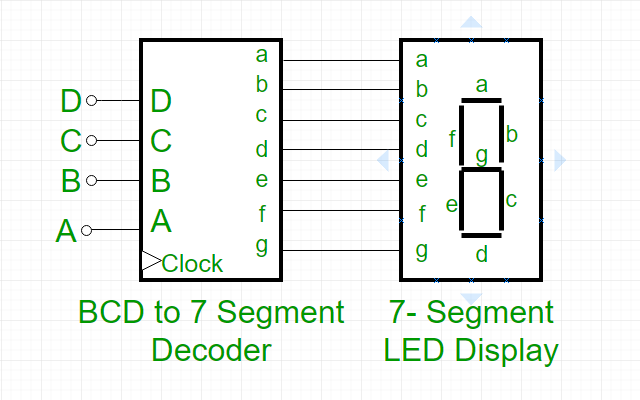
\includegraphics[width=0.5\linewidth]{bcdto7seg.png}

\section{Gray code}
A sequence of binary numbers 

\includegraphics[width=0.5\linewidth]{gray-code.pdf}

\begin{prob}
  Write all possible 3-bit binary numbers in gray-code
\end{prob}
\vspace{10em}

%\bibliography{main}
%\bibliographystyle{plain}
\end{document}
